\documentclass[12pt,a4paper]{article}
\usepackage[utf8]{inputenc}
\usepackage[T1]{fontenc}
\usepackage{amsmath}
\usepackage{geometry}
\usepackage{setspace}
\usepackage{parskip}
\usepackage{enumitem}
\usepackage{booktabs}
\usepackage{longtable}
\usepackage{array}
\usepackage{xcolor}
\usepackage{hyperref}
\usepackage{float}
\usepackage{tikz}
\usetikzlibrary{arrows.meta,positioning,calc}
\usepackage{fancyhdr}
\usepackage{titlesec}

\geometry{left=2.5cm,right=2.5cm,top=2.5cm,bottom=2.5cm,headheight=14.5pt}
\onehalfspacing
\hypersetup{colorlinks=true,linkcolor=black,urlcolor=blue,pdftitle={Resumen del Proyecto - Sistema Integral de Gestión de Eventos},pdfauthor={Daniel Cristancho, Samuel Emperador, Sebastián Sánchez, Diego Coronado}}

\definecolor{azul}{RGB}{31,78,121}
\definecolor{gris}{RGB}{242,242,242}
\definecolor{grisoscuro}{RGB}{80,80,80}
\definecolor{verde}{RGB}{39,120,70}
\definecolor{naranja}{RGB}{230,126,34}
\definecolor{morado}{RGB}{106,27,154}

\titleformat{\section}{\Large\bfseries\color{azul}}{\thesection.}{0.5em}{}
\titleformat{\subsection}{\large\bfseries}{\thesubsection.}{0.5em}{}
% Etiquetas en español (sin babel, que no está disponible en este entorno)
\renewcommand{\contentsname}{Índice}
\renewcommand{\figurename}{Figura}
\renewcommand{\tablename}{Tabla}

\pagestyle{fancy}
\fancyhf{}
\fancyhead[L]{Sistema Integral de Gestión de Eventos}
\fancyhead[R]{Resumen del Proyecto}
\fancyfoot[C]{\thepage}

\begin{document}

\begin{titlepage}
\centering
\vspace*{2cm}
{\Huge\bfseries Sistema Integral de Gestión de Eventos\par}
\vspace{0.7cm}
{\Large Arquitectura de Software\par}
\vspace{1.2cm}
{\Large\bfseries Resumen General del Proyecto --- Primera Versión\par}
\vspace{2cm}
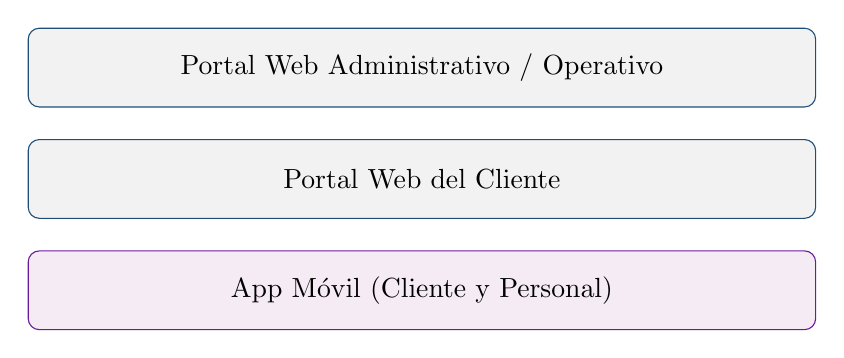
\begin{tikzpicture}
\node[draw=azul,rounded corners,fill=gris,minimum width=10cm,minimum height=1cm,align=center]
{Portal Web Administrativo / Operativo};
\node[draw=azul,rounded corners,fill=gris,minimum width=10cm,minimum height=1cm,below=0.4cm of current bounding box.south,align=center]
{Portal Web del Cliente};
\node[draw=morado,rounded corners,fill=violet!8,minimum width=10cm,minimum height=1cm,below=0.4cm of current bounding box.south,align=center]
{App Móvil (Cliente y Personal)};
\end{tikzpicture}
\vfill
\begin{tabular}{rl}
\textbf{Materia:} & Arquitectura de Software\\
\textbf{Integrantes:} & Daniel Cristancho, Samuel Emperador, Sebastián Sánchez, Diego Coronado\\
\textbf{Fecha:} & Agosto de 2026
\end{tabular}
\end{titlepage}

\tableofcontents
\newpage

\section{Idea general y problema que resuelve}

\textit{Nota de actualización (29/08/2026): al construir el prototipo de la app móvil en la
Entrega 2 se decidió unificar la App Móvil del Cliente y la App Móvil del Personal en un único
binario, con un login compartido que identifica el rol y navega al conjunto de pantallas
correspondiente (ver SAD, ADR-07). Este documento se actualiza en consecuencia.}

El proyecto centraliza en una sola plataforma todos los procesos que hoy suelen estar dispersos
en la gestión de un evento: venta de entradas, reventa, personal, parqueaderos, operación del
evento y administración general. El problema central es la \textbf{ausencia de un sistema
unificado} que coordine estos procesos de forma segura, consistente y escalable, evitando
información duplicada, errores humanos y falta de trazabilidad --- especialmente crítico cuando
hay miles de asistentes concurrentes durante la apertura de venta o el ingreso al recinto.

Esta primera versión del trabajo define explícitamente que el sistema se materializa en
\textbf{una aplicación web (con dos portales diferenciados)} y \textbf{una aplicación móvil única
(cuya navegación depende del tipo de usuario autenticado)}, todas consumiendo el mismo backend.

\section{Arquitectura de interfaces}

El sistema se divide en \textbf{tres interfaces}, cada una con un propósito y una audiencia
clara. Esto separa la lógica de negocio (que vive en el backend) de cómo cada tipo de usuario la
consume: ninguna interfaz duplica lógica, todas consumen los mismos servicios a través del API
Gateway. La App Móvil es una sola de esas tres interfaces, pero sirve a dos audiencias (Cliente y
Personal): el login identifica el rol y la navegación interna muestra el conjunto de pantallas
correspondiente.

\begin{longtable}{p{3.3cm}p{3.2cm}p{7.5cm}}
\toprule
\textbf{Interfaz} & \textbf{Usuarios} & \textbf{Qué hace}\\
\midrule
\endfirsthead
\toprule
\textbf{Interfaz} & \textbf{Usuarios} & \textbf{Qué hace}\\
\midrule
\endhead
Portal Web Administrativo / Operativo &
Administradores, organizadores, empleados con acceso de escritorio &
CRUDs del sistema, planificación de eventos, asignación y administración de personal, control de
aforo, gestión de incidentes y \textbf{emergencias/evacuaciones}, monitoreo en tiempo real.\\[0.4em]
Portal Web del Cliente &
Clientes (compradores) &
Consulta de eventos, compra de entradas, \textbf{mercado secundario} (publicar/comprar
reventas), cancelaciones y devoluciones, promociones, reserva de parqueadero.\\[0.4em]
App Móvil (Cliente y Personal) &
Clientes y empleados operativos, según el rol detectado en el login &
\textit{Rol Cliente:} visualización del \textbf{código QR} de cada entrada (función crítica para
el ingreso rápido), consulta de eventos e información, notificaciones y alertas.
\textit{Rol Personal:} consulta de turnos y asignaciones, confirmación de asignaciones, solicitud
de \textbf{cambios de turno}, \textbf{registro de ingreso/salida}, instrucciones, reporte de
incidentes y alertas de emergencia.\\
\bottomrule
\caption{Las tres interfaces del sistema y su propósito.}
\end{longtable}

\section{Actores del sistema}

\begin{itemize}
\item \textbf{Cliente:} compra, revende, reserva parqueadero.
\item \textbf{Organizador:} crea y planifica eventos, gestiona la operación.
\item \textbf{Empleado:} ejecuta labores operativas (turnos, ingreso/salida).
\item \textbf{Administrador:} gestión general (usuarios, roles, configuración).
\item \textbf{Supervisor de emergencia:} activa y coordina evacuaciones.
\item \textbf{Pasarela de pagos} y \textbf{Proveedor de notificaciones:} sistemas externos.
\end{itemize}

\section{Casos de uso asignados y su interfaz}

Estos cinco casos de uso son el aporte específico de este documento al proyecto; los demás
módulos (boletería, parqueaderos, logística, administración CRUD) son responsabilidad de otros
integrantes del equipo.

\begin{longtable}{p{3.6cm}p{6.5cm}p{4.2cm}}
\toprule
\textbf{Caso de uso} & \textbf{Qué hace} & \textbf{Interfaz principal}\\
\midrule
\endfirsthead
\toprule
\textbf{Caso de uso} & \textbf{Qué hace} & \textbf{Interfaz principal}\\
\midrule
\endhead
CU-006 --- Gestión del Mercado Secundario \textit{(complejo)} &
Reventa de entradas: publicación, compra, pago, transferencia de propiedad, invalidación y
regeneración de QR. &
Portal Web del Cliente (+ App Móvil, rol Cliente, recibe el nuevo QR).\\[0.5em]
CU-007 --- Gestión de Personal para Eventos \textit{(fusión de Administrar + Asignar Personal)} &
CRUD de empleados y asignación a eventos con validación de rol, horario y conflictos. &
Portal Web Administrativo (el empleado confirma desde la App Móvil, rol Personal).\\[0.5em]
CU-008 --- Gestionar Cambios de Turno &
Solicitud, búsqueda de reemplazo y aprobación de cambios de turno. &
App Móvil, rol Personal (solicitud) + Portal Web Administrativo (aprobación del supervisor).\\[0.5em]
CU-009 --- Registrar Ingreso y Salida del Personal &
Control de asistencia vía QR/credencial y cálculo de horas trabajadas. &
App Móvil, rol Personal.\\[0.5em]
CU-010 --- Gestionar Evacuación ante Emergencias \textit{(complejo)} &
Activación, coordinación y cierre de un protocolo de evacuación en tiempo real. &
Portal Web Administrativo (el supervisor activa y monitorea) + App Móvil (recibe
instrucciones/alertas en ambos roles).\\
\bottomrule
\caption{Casos de uso asignados, con su interfaz principal de uso.}
\end{longtable}

Nótese que \textbf{CU-010 es el único caso que toca las dos interfaces con usuarios finales a la
vez} (web administrativo para activar, la app móvil para recibir alertas, tanto en el rol Cliente
como en el rol Personal) --- es el mejor argumento para defenderlo como el caso ``no trivial'' en
infraestructura y atributos de calidad.

\section{Atributos de calidad priorizados}

\begin{longtable}{p{2.2cm}p{3cm}p{8.5cm}}
\toprule
\textbf{Prioridad} & \textbf{Atributo} & \textbf{Justificación}\\
\midrule
\endfirsthead
\toprule
\textbf{Prioridad} & \textbf{Atributo} & \textbf{Justificación}\\
\midrule
\endhead
Alta & Consistencia & Una entrada no puede tener dos dueños ni venderse dos veces.\\
Alta & Disponibilidad & Crítico durante apertura de venta, ingreso masivo y emergencias.\\
Alta & Seguridad & Datos personales, pagos, QR y permisos por rol.\\
Alta & Rendimiento & Miles de operaciones concurrentes.\\
Media-Alta & Tiempo real & Aforo, ocupación y estado de zonas durante una emergencia.\\
Media & Escalabilidad / Trazabilidad & Crecimiento por demanda y auditoría de operaciones.\\
Baja-Media & Usabilidad / Mantenibilidad / Portabilidad & Cada interfaz especializada por rol,
reduce el acoplamiento.\\
\bottomrule
\caption{Atributos de calidad y su justificación.}
\end{longtable}

\section{Arquitectura de backend}

\begin{itemize}
\item \textbf{API Gateway + balanceador de carga:} punto único de entrada, autenticación y
enrutamiento --- el mismo backend sirve a las tres interfaces sin duplicar lógica.
\item \textbf{Microservicios independientes:} Entradas/Mercado Secundario, Personal,
Eventos/Emergencias, Parqueaderos, Autenticación --- cada uno con su propia base de datos.
\item \textbf{Redis:} bloqueo temporal de concurrencia (evita doble venta) y estado de ocupación
en tiempo real.
\item \textbf{Cola de mensajes (RabbitMQ/Kafka):} desacopla generación de QR, notificaciones
push/email/SMS y liquidación de pagos.
\item \textbf{Pasarela de pagos externa:} se integra de forma asíncrona vía cola, sin bloquear la
transacción del usuario.
\end{itemize}

\begin{figure}[H]
\centering
\resizebox{0.92\textwidth}{!}{
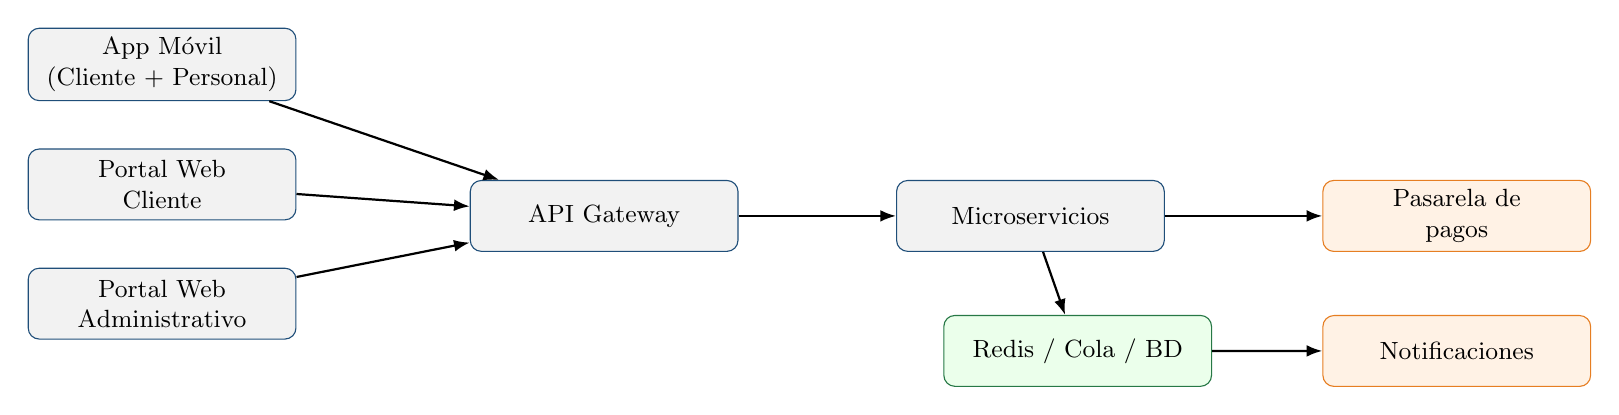
\begin{tikzpicture}[
box/.style={draw=azul,rounded corners,fill=gris,minimum width=3.4cm,minimum height=0.9cm,align=center,font=\small},
infra/.style={draw=verde,rounded corners,fill=green!8,minimum width=3.4cm,minimum height=0.9cm,align=center,font=\small},
ext/.style={draw=naranja,rounded corners,fill=orange!10,minimum width=3.4cm,minimum height=0.9cm,align=center,font=\small},
arr/.style={-{Latex[length=2mm]},thick}
]
\node[box] (am) {App Móvil\\(Cliente + Personal)};
\node[box,below=6mm of am] (wc) {Portal Web\\Cliente};
\node[box,below=6mm of wc] (wa) {Portal Web\\Administrativo};

\node[box,right=22mm of wc,yshift=-4mm] (gw) {API Gateway};
\node[box,right=20mm of gw] (ms) {Microservicios};
\node[infra,below=8mm of ms,xshift=6mm] (inf) {Redis / Cola / BD};
\node[ext,right=20mm of ms] (pg) {Pasarela de\\pagos};
\node[ext,below=8mm of pg] (no) {Notificaciones};

\foreach \x in {am,wc,wa} \draw[arr] (\x) -- (gw);
\draw[arr] (gw) -- (ms);
\draw[arr] (ms) -- (inf);
\draw[arr] (ms) -- (pg);
\draw[arr] (inf) -- (no);
\end{tikzpicture}
}
\caption{Cómo se conecta todo: las tres interfaces son distintas puertas de entrada al mismo
backend.}
\end{figure}

Las tres interfaces son distintas puertas de entrada al mismo backend: cada una expone solo las
funciones que su tipo de usuario necesita (principio de usabilidad y seguridad por rol) --- en el
caso de la App Móvil, esa especialización ocurre por navegación condicionada por rol dentro del
mismo binario, no por tener una app distinta --- pero toda la consistencia, seguridad y
trazabilidad se garantiza una sola vez, de forma centralizada, en los microservicios detrás del
Gateway.

\section{Documentación entregada (modelo C4)}

\begin{itemize}
\item \textbf{Nivel 1 (Contexto):} el sistema como caja negra frente a los cinco roles de usuario
y los dos sistemas externos.
\item \textbf{Nivel 2 (Contenedores):} zoom a las tres interfaces, el API Gateway, los
microservicios y la infraestructura.
\item \textbf{Nivel 3 (Componentes):} zoom interno al Servicio de Entradas y Mercado Secundario
(el caso complejo CU-006).
\end{itemize}

Cada diagrama fue validado contra el checklist oficial de
\href{https://c4model.com/diagrams/checklist}{c4model.com/diagrams/checklist} (título, tipo,
alcance, leyenda y tecnología de cada relación), y se documenta en el archivo separado
\textit{Diagramas de Arquitectura --- Modelo C4}.

\section{Conclusión}

Esta primera versión del proyecto define con claridad tres superficies de interacción --- dos
portales web y una aplicación móvil única, cuya navegación se especializa según el rol
autenticado (Cliente o Personal) --- todas apoyadas en un único backend de microservicios. Los
cinco casos de uso asignados (CU-006 a CU-010) cubren de forma cohesiva el ciclo completo del
personal operativo (administración, asignación, cambios de turno, asistencia) y el proceso más
complejo del sistema desde el punto de vista arquitectónico: la reventa segura de entradas. La
incorporación explícita de las tres interfaces refuerza la justificación de atributos como
disponibilidad, seguridad, tiempo real y usabilidad, y deja una base clara para iterar en
próximas versiones del trabajo.

\end{document}
